\documentclass{article}
\usepackage[a4paper, total={7in, 10in}]{geometry}
\usepackage{listings}
\usepackage{amsmath}
\usepackage{url}
\usepackage{float}
\usepackage{enumitem}
\usepackage{listings}
\usepackage{setspace}
\usepackage{textcomp}
\usepackage{mathtools}
\usepackage{amssymb}
\usepackage[T1]{fontenc}

\title{\Huge Lista 2 - Soluções}
\author{\Large Arquitetura e Organização de Computadores}
\date{Maio 2024}

\begin{document}

\maketitle

\large
Qual número é armazenado como \verb|0x49179EA0| conforme a norma IEEE 754?
\verb|62.1034E4|

\bigskip
\bigbreak

Quais valores hexadecimais podem representar o número \verb|3.462408E-11| conforme a norma IEEE 754?
\begin{align*}
&3.462408E-11 = 1.18967433003270144*2^{-35} \\ 
&\text{MSb} = 0 \\
&\text{exp} = 127 - 35 = 92 = 0b01011100 \\
&16*0.18967433003270144 = 3.03478928052322304  \rightarrow 3 \\
&16*0.03478928052322304 = 0.55662848837156864  \rightarrow 0 \\
&16*0.55662848837156864 = 8.90605581394509824  \rightarrow 8 \\
&16*0.90605581394509824 = 14.49689302312157184 \rightarrow E \\
&16*0.49689302312157184 = 7.95028836994514944  \rightarrow 7 \\
&16*0.95028836994514944 = 15.20461391912239104 \rightarrow F \\
&0x308E7F = 0b001100001000111001111111 \\
&\text{concatena(MSb, exp, mantissa)} = 0b001011100001100001000111001111111 \\
&\text{se descarta o bit menos significativo,} \\
&0b00101110000110000100011100111111 \\
&0x2E18473F \\
&\text{se arredonda o bit menos significativo,} \\
&0b00101110000110000100011101000000 \\
&0x2E184740
\end{align*}
\verb|0x2E184740| e \verb|0x2E18473F|

\bigskip
\bigbreak

Traduza o programa abaixo, em C, para MIPS.
\begin{center}
    \begin{minipage}{0.6\textwidth}
        \begin{lstlisting}[frame=single]
int factorial(int n) {
	if(n == 0) return 1;
	return n * factorial(n - 1);
}

void main()  {
	int num = 5;
        int fact = factorial(num);
}
        \end{lstlisting}
    \end{minipage}
\end{center}

\url{https://github.com/Eduardo-bat/AOC_2024/blob/main/factorial.asm}

\pagebreak

Ao fim da execução do programa abaixo, quais os valores em \verb|$sp| e \verb|$s1|?  Qual o menor valor armazenado, ao longo da execução deste programa, em \verb|$sp|?

\begin{center}
    \begin{minipage}{0.35\textwidth}
        \begin{lstlisting}[frame=single]
j main

recursive:
lw $t0, 0($sp)
addi $sp, $sp, 4

bne $t0, $0, else
addi $sp, $sp, -4
sw $t0, 0($sp)
jr $ra

else:
addi $t0, $t0, -1
addi $sp, $sp, -8
sw $t0, 0($sp)
sw $ra, 4($sp)
jal recursive
lw $t0, 0($sp)
lw $ra, 4($sp)
addi $sp, $sp, 8
addi $t0, $t0, 1
addi $sp, $sp, -4
sw $t0, 0($sp)
jr $ra

main:
addi $s0, $0, 0xABCD
addi $sp, $sp, -4
sw $s0, 0($sp)
jal recursive
lw $s1, 0($sp)
addi $sp, $sp, 4
        \end{lstlisting}
    \end{minipage}
\end{center}

\url{https://github.com/Eduardo-bat/AOC_2024/blob/main/recursive.asm}

\pagebreak

Traduza o programa abaixo, em C, para MIPS.

\begin{center}
    \begin{minipage}{0.475\textwidth}
        \begin{lstlisting}[frame=single]
#include <math.h>

float fop(float a, float b) {
    if(b == 0) return NAN;
    return a*b + a/b;
}

void main() {
    float a = 40.1;
    float b = 00.4;
    float c = fop(a, b);
}
        \end{lstlisting}
    \end{minipage}
\end{center}

\url{https://github.com/Eduardo-bat/AOC_2024/blob/main/float.asm}

\bigbreak
\normalsize

{\large Como \verb|PC| é tratado no estágio \textbf{Fetch}? Em quais condições seu valor não pode ser atualizado?\vspace{1mm}}

\noindent Em cada estágio \textbf{Fetch}, \verb|PC'| é armazenado no registrador de \verb|PC| e transmitido à memória de instruções. Além disso, seu valor é incrementado e o resultado é disponibilizado para o multiplexador que define o próximo \verb|PC'| e para o registrador F/D. Quando a necessidade de um stall é detectada no estágio \textbf{Decode} de uma instrução, o \textbf{Fetch} da próxima deve ser postergado para o próximo ciclo. Neste caso, a escrita no registrador de \verb|PC| é bloqueada. Isto mantém impede que \verb|PC| seja incrementado por um ciclo de clock (o mesmo em que a necessidade de stall é detectada), reabilitando o fluxo normal no próximo.
\bigbreak

{\large Em qual estágio a tratativa de data hazards para \verb|lw| é feita? Qual condição é verificada nesta tratativa? Quando este tipo de hazard é detectado, como é tratado?\vspace{1mm}}

\noindent A tratativa de data hazards para \verb|lw| é feita no estágio \textbf{Decode}. Neste, \verb|rs| e \verb|rt| são transmitidos à unidade de hazards, que,\\
- para cada endereço, se este for igual ao endereço de destino da instrução anterior \textbf{e} a instrução anterior for \verb|lw|, mantém a instrução neste estágio, impedindo a escrita no registrador de \verb|PC| e no registrador F/D e forçando todos os sinais em D/E para 0.
\bigbreak

{\large Descreva como, no estágio \textbf{Execute}, é feita a avaliação e tratativa de hazards.\vspace{1mm}}

\noindent Os endereços dos registradores usados nesta instrução são transmitidos à unidade de hazards, que,\\
- para cada endereço, se este for igual ao endereço de destino de alguma das duas instruções anteriores,\\
--- se a última instrução modifica o banco de registradores, seleciona o resultado desta como valor correspondente ao endereço,\\
--- senão, se a penúltima instrução modifica o banco de registradores, seleciona o resultado desta como valor correspondente ao endereço,\\
- senão, seleciona o valor contido no banco como valor correspondente ao endereço.\\
O endereço do registrador de destino e os sinais de controle da memória são transmitidos à unidade de hazards, para permitir decisões em instruções posteriores;
\bigbreak

{\large Quais sinais, no estágio \textbf{Memory}, contribuem para a detecção ou tratativa de hazards? Como estes são avaliados ou utilizados?\vspace{1mm}}

\noindent Neste estágio, \verb|ALUOutM| é disponibilizado para ser usado como operando no estágio \textbf{Execute} da próxima instrução e para comparação no estágio \textbf{Decode} da posterior a esta. Além disso, \verb|WriteRegM| e \verb|RegWriteM| são transmitidos à hazard unit para avaliação de hazards no estágio \textbf{Execute} da próxima instrução.
\bigbreak

{\large Quais sinais, no estágio \textbf{WriteBack}, contribuem para a detecção ou tratativa de hazards? Como estes são avaliados ou utilizados?\vspace{1mm}}

\noindent Neste estágio, \verb|ALUOutW| é disponibilizado para ser usado como operando no estágio \textbf{Execute} da instrução que sucede a próxima. Além disso, \verb|WriteRegW| e \verb|RegWriteW| são transmitidos à hazard unit para avaliação de hazards no estágio \textbf{Execute} desta.
\bigbreak

{\large Em qual estágio de uma instrução \verb|beq| os hazards pertinentes a ela são detectados? Como estes são avaliados e tratados?\vspace{1mm}}

\noindent Os hazards pertinentes à instrução \verb|beq| são detectados no estágio \textbf{Decode} desta:\\
- se a última instrução for \verb|lw| e esta atualizar um dos endereços fonte para a comparação, \verb|beq| é mantida em \textbf{Decode} por dois ciclos de clock, já que a instrução anterior estará em \textbf{Execute} e o valor só estará disponível em \textbf{WriteBack};\\
- senão, se a última instrução for de tipo lógica/aritmética e esta atualizar um dos endereços fonte para a comparação ou a penúltima for \verb|lw| e esta atualizar um dos endereços fonte para a comparação, \verb|beq| é mantida em \textbf{Decode} por um ciclo de clock;\\
- senão, se a penúltima instrução for lógica/aritmética e esta atualizar um dos endereços fonte para a comparação, \verb|ALUOutM| substitui o valor armazenado no endereço coincidente;
\bigbreak

{\large Em um processador pipeline, o que significa, "limpar" ou "resetar" um registrador de pipeline? Como isso impede a continuação da instrução a partir do estágio em que ocorre \vspace{1mm}}

\noindent "Limpar" ou "resetar" um registrador de pipeline corresponde a forçar o valor 0 em todos os sinais armazenados nele. Isso impede a propagação da instrução porque desabilita a escrita em todos os componentes posteriores e acessa, restritamente, o endereço 0 do banco de registradores, habilitado somente para leitura.
\bigbreak

{\large No processador pipeline implementado no livro de referência, é possível realizar forwarding do estágio \textbf{WriteBack} para o estágio \textbf{Memory}? Em qual condição isto é necessário? Qual a justificativa para a decisão tomada na implementação apresentada pelo livro?\vspace{1mm}}

\noindent Não é possível. Quando uma \verb|sw| é executada logo após uma instrução lógica/aritmética que escreve no registrador a ser armazenado na memória. Não sei a justificativa.
\bigbreak

\begin{center}
    \begin{minipage}{0.475\textwidth}
        \begin{lstlisting}[frame=single]
i00: addi $s0, $0, 10
i01: sw   $s0, 0($sp)
i02: addi $s0, $0, 2
i03: addi $s1, $0, 3
i04: add  $s2, $s1, $s0
i05: sub  $s1, $s2, $s0
i06: lw   $s3, 0($sp)
i07: add  $s4, $s3, $s3
i08: beq  $s4, $s3, one
i09: add  $s0, $0, $0
i10: add  $s1, $0, $0
i11: add  $s2, $0, $0
i12: add  $s3, $0, $0
i13: beq  $0, $0, zero
one:
i14: add  $s0, $0, 1
i15: add  $s1, $0, 1
i16: add  $s2, $0, 1
i17: add  $s3, $0, 1
zero:
i18: add  $s6, $s2, $s3
i19: add  $s5, $s0, $s1
i20: add  $s7, $s6, $s5
        \end{lstlisting}
    \end{minipage}
\end{center}

\pagebreak

{\large Considerando uma arquitetura que detecte hazards, empregue stall e previsão de desvio (assume que não é tomado), mas não empregue forwarding, indique, na tabela abaixo, em qual estágio cada instrução está em cada ciclo de clock.}

\begin{table}[H]
\begin{tabular}{|l|l|l|l|l|l|l|l|l|l|l|l|l|l|l|l|l|}
\hline
inst & C0  & C1  & C2  & C3  & C4  & C5  & C6  & C7  & C8  & C9  & C10 & C11 & C12 & C13 & C14 & C15 \\ \hline
i0:  &  F  &  D  &  E  &  M  &  W  &     &     &     &     &     &     &     &     &     &     &     \\ \hline
i1:  &     &  F  &  D  &  D  &  D  &  E  &  M  &  W  &     &     &     &     &     &     &     &     \\ \hline
i2:  &     &     &     &     &  F  &  D  &  E  &  M  &  W  &     &     &     &     &     &     &     \\ \hline
i3:  &     &     &     &     &     &  F  &  D  &  E  &  M  &  W  &     &     &     &     &     &     \\ \hline
i4:  &     &     &     &     &     &     &  F  &  D  &  D  &  D  &  E  &  M  &  W  &     &     &     \\ \hline
i5:  &     &     &     &     &     &     &     &     &     &  F  &  D  &  D  &  D  &  E  &  M  &  W  \\ \hline
inst & C12 & C13 & C14 & C15 & C16 & C17 & C18 & C19 & C20 & C21 & C22 & C23 & C24 & C25 & C26 & C27 \\ \hline
i6:  &  F  &  D  &  E  &  M  &  W  &     &     &     &     &     &     &     &     &     &     &     \\ \hline
i7:  &     &  F  &  D  &  D  &  D  &  E  &  M  &  W  &     &     &     &     &     &     &     &     \\ \hline
i8:  &     &     &     &     &  F  &  D  &  D  &  D  &  E  &  M  &  W  &     &     &     &     &     \\ \hline
i9:  &     &     &     &     &     &     &     &  F  &  D  &  E  &  M  &  W  &     &     &     &     \\ \hline
i10: &     &     &     &     &     &     &     &     &  F  &  D  &  E  &  M  &  W  &     &     &     \\ \hline
i11: &     &     &     &     &     &     &     &     &     &  F  &  D  &  E  &  M  &  W  &     &     \\ \hline
i12: &     &     &     &     &     &     &     &     &     &     &  F  &  D  &  E  &  M  &  W  &      \\ \hline
inst & C23 & C24 & C25 & C26 & C27 & C28 & C29 & C30 & C31 & C32 & C33 & C34 & C35 & C36 & C37 & C38 \\ \hline
i13: &  F  &  D  &  E  &  M  &  W  &     &     &     &     &     &     &     &     &     &     &     \\ \hline
i14: &     &  F  &  -  &  -  &  -  &  -  &     &     &     &     &     &     &     &     &     &     \\ \hline
i18: &     &     &  F  &  D  &  E  &  M  &  W  &     &     &     &     &     &     &     &     &     \\ \hline
i19: &     &     &     &  F  &  D  &  E  &  M  &  W  &     &     &     &     &     &     &     &     \\ \hline
i20: &     &     &     &     &  F  &  D  &  D  &  D  &  E  &  M  &  W  &     &     &     &     &     \\ \hline
\end{tabular}
\end{table}


\pagebreak

{\large Considerando uma arquitetura que detecte hazards e empregue forwarding, stall e previsão de desvio (assume que não é tomado) indique, na tabela abaixo, em qual estágio cada instrução está em cada ciclo de clock. Neste exercício, não se restrinja ao processador implementado no livro. Indique os recursos que achar pertinentes.}

No processador que decidi usar, há forwarding WB\textrightarrow MEM para tratar instruções \verb|sw| antecedidas diretamente por instruções que escrevem no registrador a ser armazenado. Uma seta vertical indica que o estágio é fonte de um forwarding. Uma seta horizontal indica que o estágio recebe forwarding.
\begin{table}[H]
\begin{tabular}{|l|l|l|l|l|l|l|l|l|l|l|l|l|l|l|l|l|}
\hline
inst & C0  & C1  & C2  & C3  & C4  & C5  & C6  & C7  & C8  & C9  & C10 & C11 & C12 & C13 & C14 & C15 \\ \hline
i0:  &  F  &  D  &  E  &  M  &$\downarrow$W  &     &     &     &     &     &     &     &     &     &     &     \\ \hline
i1:  &     &  F  &  D  &  E  &$\rightarrow$M  &  W  &     &     &     &     &     &     &     &     &     &     \\ \hline
i2:  &     &     &  F  &  D  &  E  &  M  &$\downarrow$W  &     &     &     &     &     &     &     &     &     \\ \hline
i3:  &     &     &     &  F  &  D  &  E  &$\downarrow$M  &  W  &     &     &     &     &     &     &     &     \\ \hline
i4:  &     &     &     &     &  F  &  D  &$\rightrightarrows$E  &$\downarrow$M  &  W  &     &     &     &     &     &     &     \\ \hline
i5:  &     &     &     &     &     &  F  &  D  &$\rightarrow$E  &  M  &  W  &     &     &     &     &     &     \\ \hline
i6:  &     &     &     &     &     &     &  F  &  D  &  E  &  M  &$\downarrow$W  &     &     &     &     &     \\ \hline
i7:  &     &     &     &     &     &     &     &  F  &  D  &  D  &$\rightarrow$E  &$\downarrow$M  &  W  &     &     &     \\ \hline
i8:  &     &     &     &     &     &     &     &     &     &  F  &  D  &$\rightarrow$D  &  E  &  M  &  W  &     \\ \hline
i9:  &     &     &     &     &     &     &     &     &     &     &     &  F  &  D  &  E  &  M  &  W  \\ \hline
inst & C12 & C13 & C14 & C15 & C16 & C17 & C18 & C19 & C20 & C21 & C22 & C23 & C24 & C25 & C26 & C27 \\ \hline
i10: &  F  &  D  &  E  &  M  &  W  &     &     &     &     &     &     &     &     &     &     &     \\ \hline
i11: &     &  F  &  D  &  E  &  M  &  W  &     &     &     &     &     &     &     &     &     &     \\ \hline
i12: &     &     &  F  &  D  &  E  &  M  &  W  &     &     &     &     &     &     &     &     &     \\ \hline
i13: &     &     &     &  F  &  D  &  E  &  M  &  W  &     &     &     &     &     &     &     &     \\ \hline
i14: &     &     &     &     &  F  &  -  &  -  &  -  &  -  &     &     &     &     &     &     &     \\ \hline
i18: &     &     &     &     &     &  F  &  D  &  E  &  M  &$\downarrow$W  &     &     &     &     &     &     \\ \hline
i19: &     &     &     &     &     &     &  F  &  D  &  E  &$\downarrow$M  &  W  &     &     &     &     &     \\ \hline
i20: &     &     &     &     &     &     &     &  F  &  D  &$\rightrightarrows$E  &  M  &  W  &     &     &     &     \\ \hline
\end{tabular}
\end{table}

{\large Reorganize o programa a seguir a fim de evitar hazards sem alterar seu estado final.}

\begin{center}
    \begin{minipage}{0.25\textwidth}
        \begin{lstlisting}[frame=single]
or   $t2, $t1, $t0
nor  $t9, $t8, $t7
addi $s2, $s1, 1
add  $s2, $s1, $s0
sub  $s4, $s3, $s2
xor  $t2, $t1, $t0
sw   $t2, 0($sp)
lw   $t9, 4($sp)
subi $t0, $t0, 1
and  $t7, $t8, $t9
        \end{lstlisting}
    \end{minipage}
\end{center}

\begin{center}
    \begin{minipage}{0.25\textwidth}
        \begin{lstlisting}[frame=single]
nor  $t9, $t8, $t7
lw   $t9, 4($sp)
addi $s2, $s1, 1
add  $s2, $s1, $s0
or   $t2, $t1, $t0
xor  $t2, $t1, $t0
subi $t0, $t0, 1
and  $t7, $t8, $t9
sub  $s4, $s3, $s2
sw   $t2, 0($sp)
        \end{lstlisting}
    \end{minipage}
\end{center}

{\large Mostre como as seguintes instruções são executadas em um processador de ciclo único. Para isso, indique quais sinais são transferidos entre quais componentes.}

\begin{enumerate}
    \item sub\\

\begin{figure}[H]
    \centering
    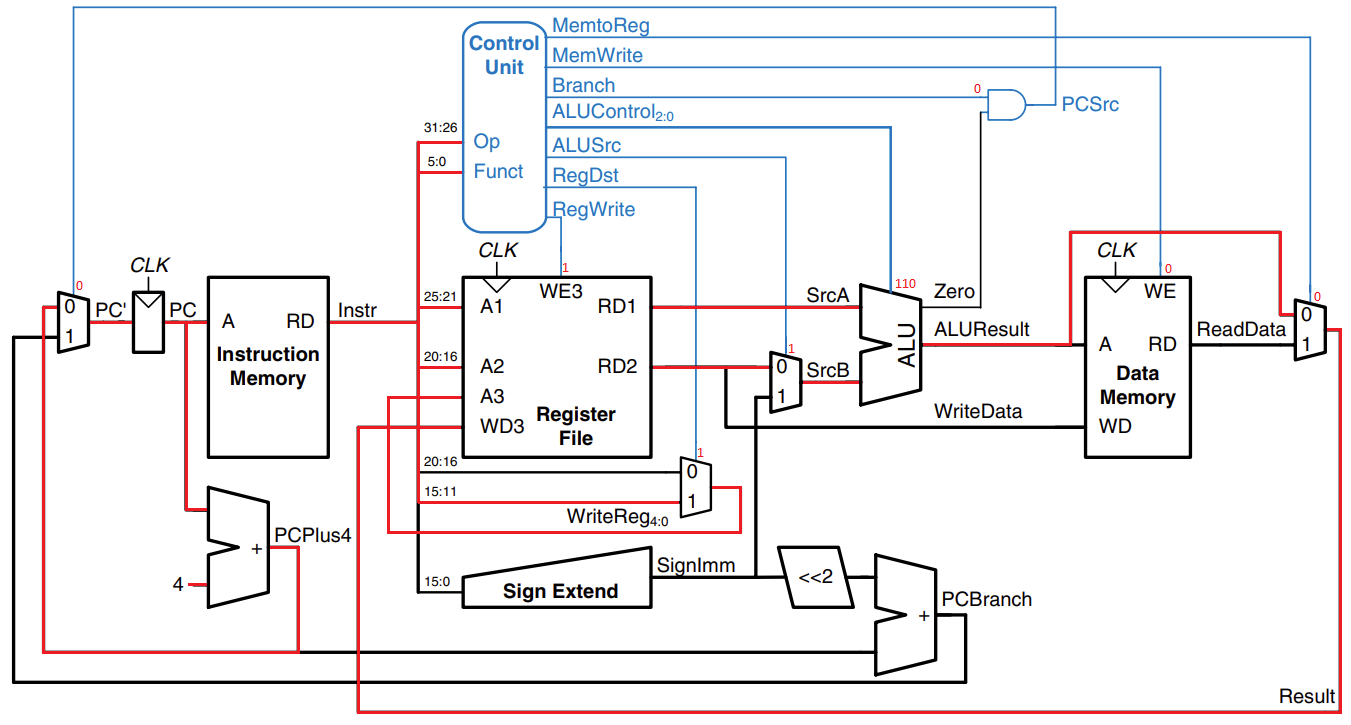
\includegraphics[width=1\linewidth]{sub.png}
\end{figure}

    \item jr\\

\begin{figure}[H]
    \centering
    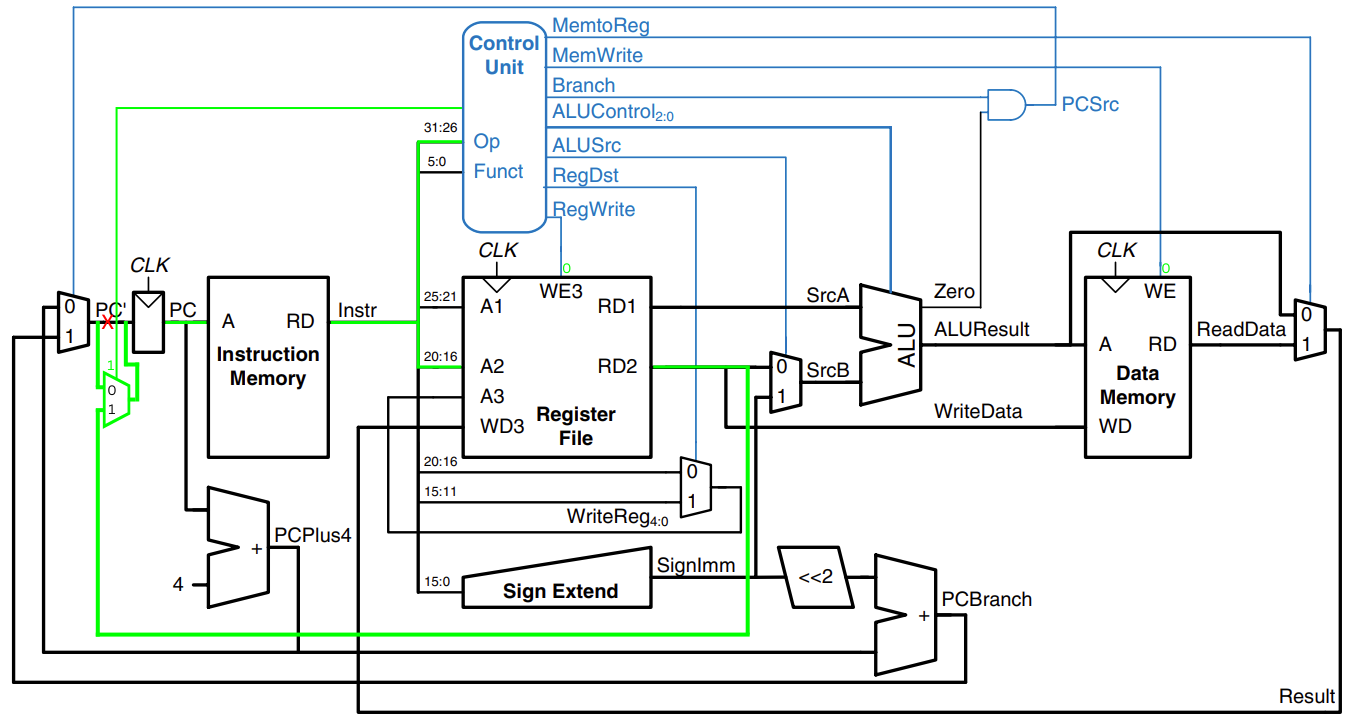
\includegraphics[width=1\linewidth]{jr.png}
\end{figure}

    \item jal\\

\begin{figure}[H]
    \centering
    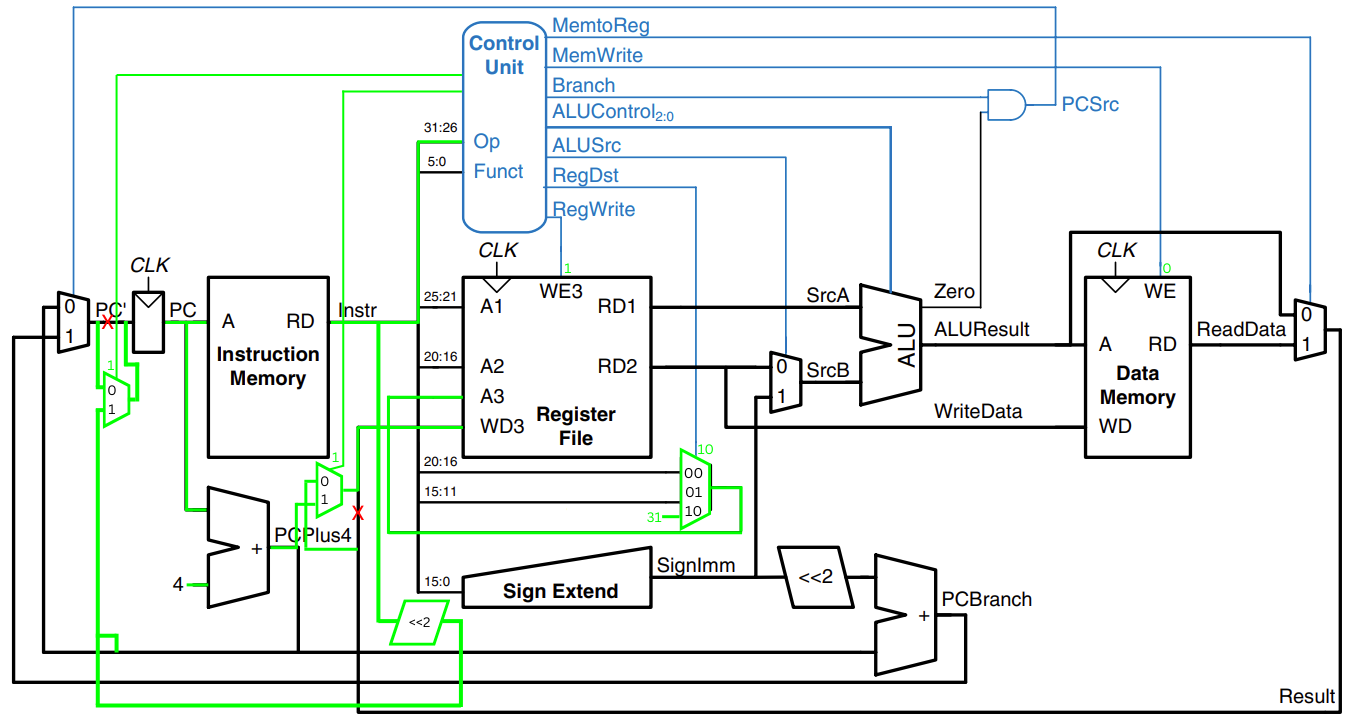
\includegraphics[width=1\linewidth]{jal.png}
\end{figure}

    \item beq\\

\begin{figure}[H]
    \centering
    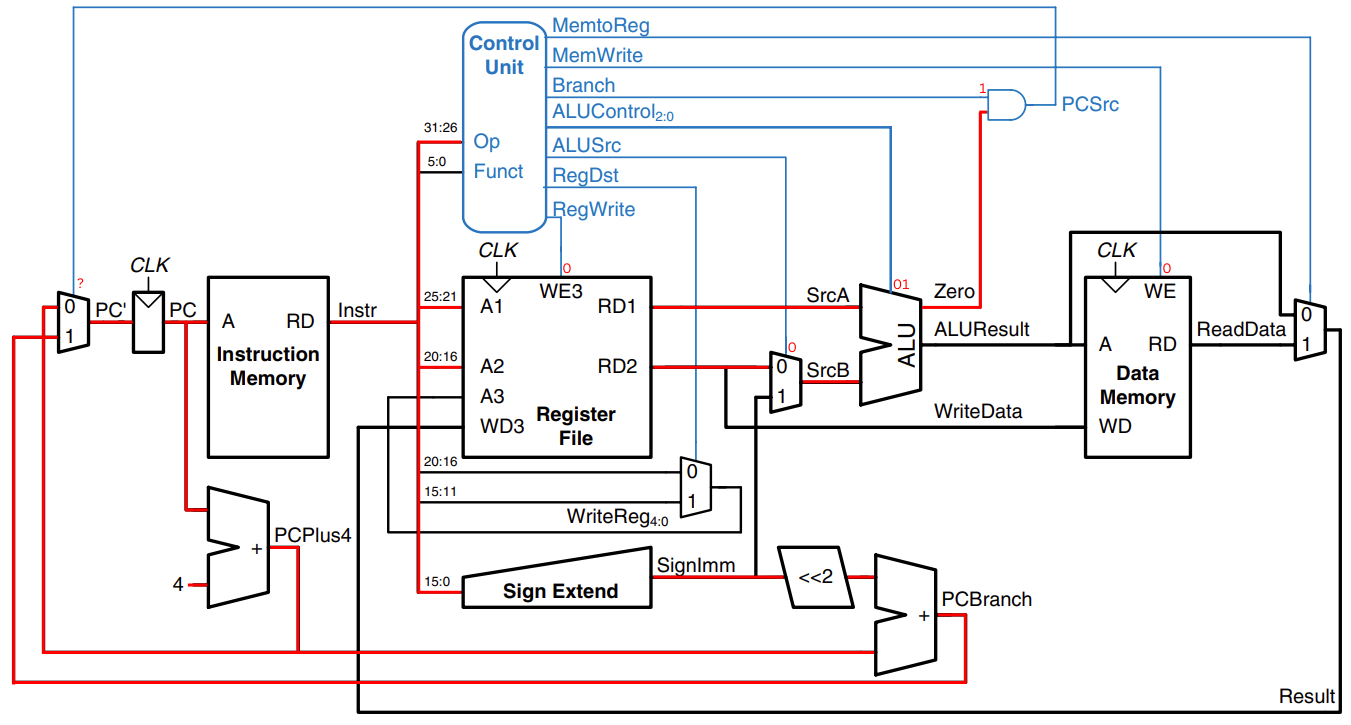
\includegraphics[width=1\linewidth]{beq.png}
\end{figure}

    \item sw\\

\begin{figure}[H]
    \centering
    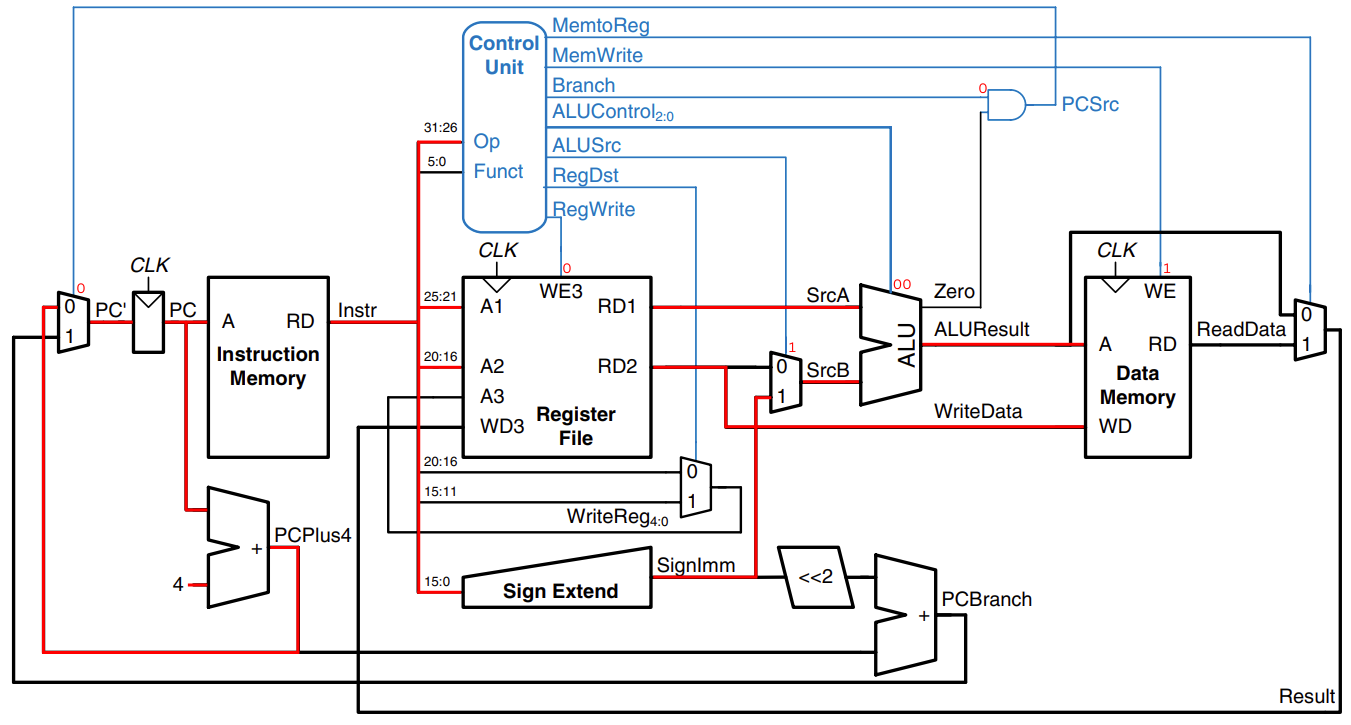
\includegraphics[width=1\linewidth]{sw.png}
\end{figure}

    \item lw\\

\begin{figure}[H]
    \centering
    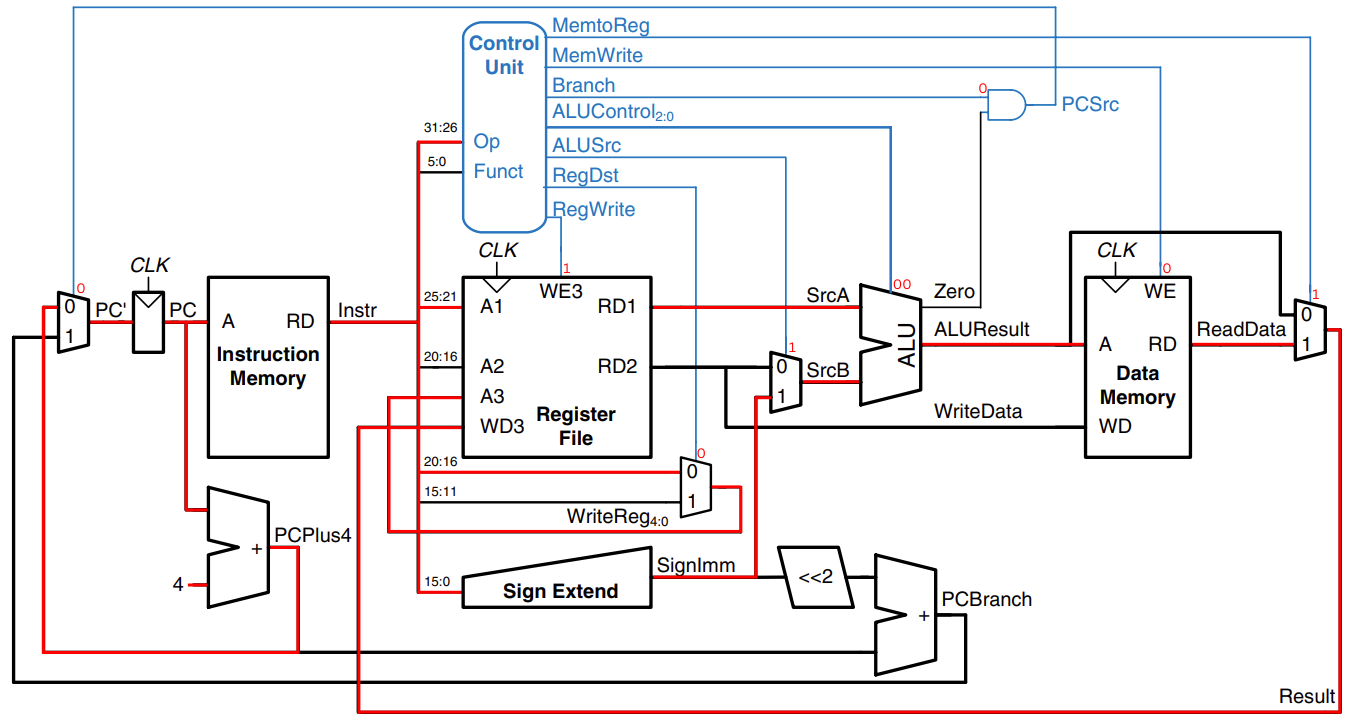
\includegraphics[width=1\linewidth]{lw.png}
\end{figure}

    \item addi\\

\begin{figure}[H]
    \centering
    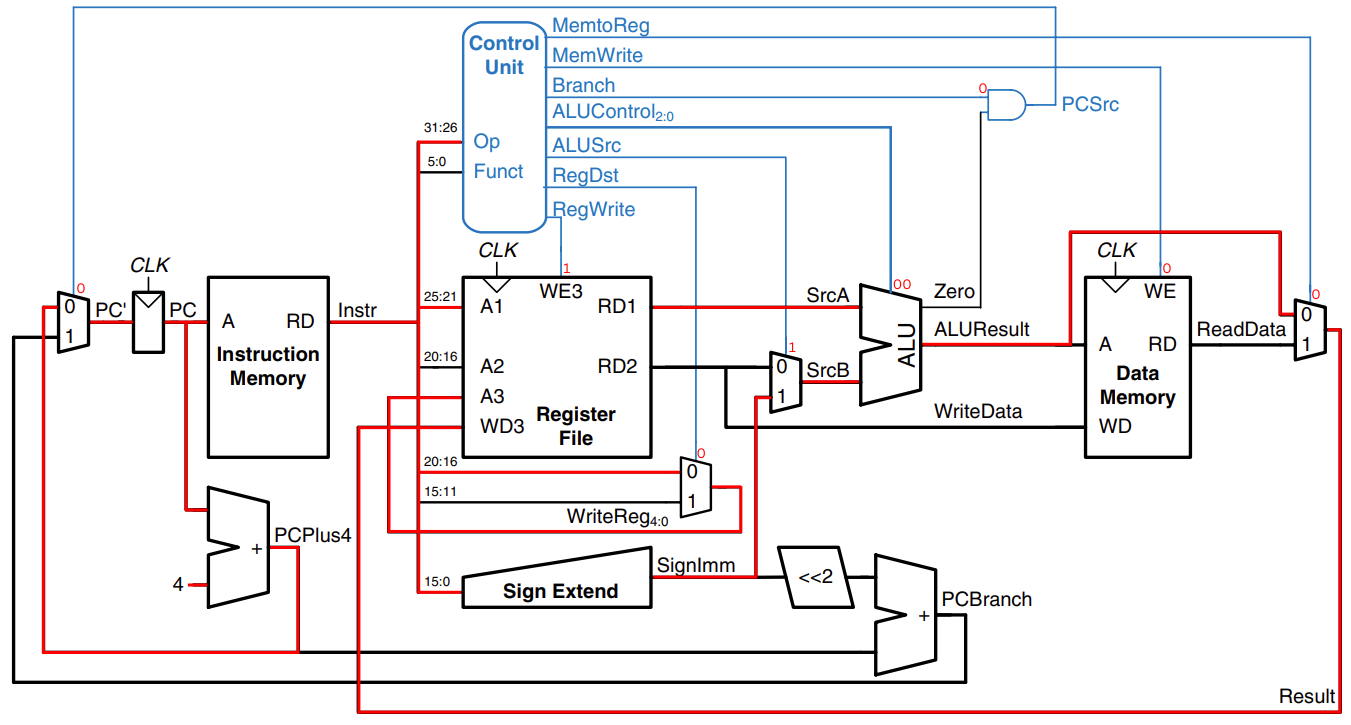
\includegraphics[width=1\linewidth]{addi.png}
\end{figure}

\end{enumerate}

{\large Descreva, temporalmente, como as seguintes instruções são executadas em um processador multi-ciclo. Para isso, indique quais sinais são transferidos entre quais componentes.}

\begin{enumerate}
    \item sub\\
1 $\text{PC}_\text{reg} \xrightarrow{\text{PC}} \text{Adr}_\text{multiplexer} \xrightarrow{\text{Adr}} \text{Mem} \xrightarrow{\text{Instr/Data}} \text{InstReg}$, $\text{CtrlUnit} \begin{matrix*}[l] 
\xrightarrow{\text{PC}_\text{write}} \text{PCEn}_\text{OR} \xrightarrow{\text{PCEn}} \text{PC}_\text{reg} \\ 
\xrightarrow{\text{PCSrc}} \text{PCSrc}_\text{multiplexer} \\
\xrightarrow{\text{IR}_\text{write}} \text{InstReg} \\
\xrightarrow{\text{IorD}} \text{Adr}_\text{multiplexer} \\ \xrightarrow{\text{ALUSrcA}} \text{SrcA}_\text{multiplexer} \\ \xrightarrow{\text{ALUSrcB}} \text{SrcB}_\text{multiplexer} \\ \xrightarrow{\text{PCSrc}} \text{PCSrc}_\text{multiplexer} \end{matrix*}$,\\ $\begin{matrix*}[r] \text{PC}_\text{reg} \xrightarrow{\text{PC}} \text{SrcA}_\text{multiplexer} \xrightarrow{\text{SrcA}} \\ \text{4} \xrightarrow{\text{4}} \text{SrcB}_\text{multiplexer} \xrightarrow{\text{SrcB}}\end{matrix*} \text{ALU} \xrightarrow{\text{PC+4}} \text{PCSrc}_\text{multiplexer} \xrightarrow{\text{PC+4}} \text{PC}_\text{reg}$\\

\bigbreak

2 $\text{InstReg} \begin{matrix*}[l] 
\xrightarrow{\text{Funct \& Op}} \text{CtrlUnit} \\ \xrightarrow{\text{rt \& rs}} \text{RegFile} \xrightarrow{\text{rd1 \& rd2}} \text{RegFileData}_\text{reg} \end{matrix*}$\\

\bigbreak

3 $\text{RegFileData}_\text{reg} \begin{matrix*}[l] \xrightarrow{\text{A}} \text{SrcA}_\text{multiplexer} \xrightarrow{\text{SrcA}} \\ \xrightarrow{\text{B}} \text{SrcB}_\text{multiplexer} \xrightarrow{\text{SrcB}} \end{matrix*} \text{ALU} \xrightarrow{\text{ALURes}} \text{ALUOut}_\text{reg}$, $\text{CtrlUnit} \begin{matrix*}[l] 
\xrightarrow{\text{ALUCtrl}} \text{ALU} \\ \xrightarrow{\text{ALUSrcA}} \text{SrcA}_\text{multiplexer} \\ \xrightarrow{\text{ALUSrcB}} \text{SrcB}_\text{multiplexer} \end{matrix*}$\\

\bigbreak

4 $\text{ALUOut}_\text{reg} \xrightarrow{\text{ALUOut}} \text{WD3}_\text{multiplexer} \xrightarrow{\text{ALUOut}} \text{WD3}_\text{RegFile}$,  $\text{CtrlUnit} \begin{matrix*}[l] 
\xrightarrow{\text{RegDst}} \text{RegDst}_\text{multiplexer} \\ \xrightarrow{\text{MemtoReg}} \text{WD3}_\text{multiplexer} \\ \xrightarrow{\text{RegWrite}} \text{RegFile} \end{matrix*}$\\

\bigbreak

    \item jr\\

3.\\
CtrlUnit -> \{PCSrc\} -> PCSrcMult;\\
CtrlUnit -> \{PCWrite\} -> PCreg;\\
RegFileReg -> \{A\} -> PCSrcMult -> \{A\} -> PCReg;\\

\bigbreak

    \item jal\\

2.\\
CtrlUnit -> \{PCSrc\} -> PCSrcMult;\\
CtrlUnit -> \{PCWrite\} -> PCreg;\\
\{PC[31:28] concat Imm < < 2\} -> PCSrcMult;\\
CtrlUnit -> \{WriteSrc\} -> WD3Mult;\\
\{31\} -> WD3Mult -> RegFile

\bigbreak

    \item beq (interessante: o endereço de desvio é computado em Decode e a igualdade verificada no execute)\\

1 $\text{PC}_\text{reg} \xrightarrow{\text{PC}} \text{Adr}_\text{multiplexer} \xrightarrow{\text{Adr}} \text{Mem} \xrightarrow{\text{Instr/Data}} \text{InstReg}$, $\text{CtrlUnit} \begin{matrix*}[l] 
\xrightarrow{\text{PC}_\text{write}} \text{PCEn}_\text{OR} \xrightarrow{\text{PCEn}} \text{PC}_\text{reg} \\ 
\xrightarrow{\text{PCSrc}} \text{PCSrc}_\text{multiplexer} \\
\xrightarrow{\text{IR}_\text{write}} \text{InstReg} \\
\xrightarrow{\text{IorD}} \text{Adr}_\text{multiplexer} \\ \xrightarrow{\text{ALUSrcA}} \text{SrcA}_\text{multiplexer} \\ \xrightarrow{\text{ALUSrcB}} \text{SrcB}_\text{multiplexer} \\ \xrightarrow{\text{PCSrc}} \text{PCSrc}_\text{multiplexer} \end{matrix*}$,\\ $\begin{matrix*}[r] \text{PC}_\text{reg} \xrightarrow{\text{PC}} \text{SrcA}_\text{multiplexer} \xrightarrow{\text{SrcA}} \\ \text{4} \xrightarrow{\text{4}} \text{SrcB}_\text{multiplexer} \xrightarrow{\text{SrcB}}\end{matrix*} \text{ALU} \xrightarrow{\text{PC+4}} \text{PCSrc}_\text{multiplexer} \xrightarrow{\text{PC+4}} \text{PC}_\text{reg}$\\

\bigbreak

2 $\text{InstReg} \begin{matrix*}[l] 
\xrightarrow{\text{Funct \& Op}} \text{CtrlUnit} \\ \xrightarrow{\text{rt \& rs}} \text{RegFile} \xrightarrow{\text{rd1 \& rd2}} \text{RegFileData}_\text{reg}\\
\xrightarrow{\text{Imm}} \text{ImmExt} \xrightarrow{\text{SignImm}} \text{ImmShift} \xrightarrow{\text{ShiftImm}} \text{SrcB}_\text{multiplexer} \end{matrix*}$, $\text{PC}_\text{reg} \xrightarrow{\text{PC}} \text{SrcA}_\text{multiplexer}$,
\smallbreak
$\text{CtrlUnit} \begin{matrix*}[l] 
\xrightarrow{\text{ALUCtrl}} \text{ALU} \\ \xrightarrow{\text{ALUSrcA}} \text{SrcA}_\text{multiplexer} \\ \xrightarrow{\text{ALUSrcB}} \text{SrcB}_\text{multiplexer} \end{matrix*}$, $\begin{matrix*}[r] \text{SrcA}_\text{multiplexer} \xrightarrow{\text{PC}} \\  \text{SrcB}_\text{multiplexer} \xrightarrow{\text{ShiftImm}}\end{matrix*} \text{ALU} \xrightarrow{\text{PCBranch}} \text{PCSrc}_\text{multiplexer}$\\

3 $\text{RegFileData}_\text{reg} \begin{matrix*}[l] \xrightarrow{\text{A}} \text{SrcA}_\text{multiplexer} \xrightarrow{\text{SrcA}} \\ \xrightarrow{\text{B}} \text{SrcB}_\text{multiplexer} \xrightarrow{\text{SrcB}} \end{matrix*} \text{ALU} \xrightarrow{\text{Zero}} \text{Branch}_\text{AND}$, $\text{CtrlUnit} \begin{matrix*}[l] \xrightarrow{\text{Branch}} \text{Branch}_\text{AND} \\ \xrightarrow{\text{PCSrc}} \text{PCSrc}_\text{multiplexer} \\
\xrightarrow{\text{ALUCtrl}} \text{ALU} \\ \xrightarrow{\text{ALUSrcA}} \text{SrcA}_\text{multiplexer} \\ \xrightarrow{\text{ALUSrcB}} \text{SrcB}_\text{multiplexer} \end{matrix*}$,\\
$\begin{matrix*}[r] \text{PCSrc}_\text{multiplexer} \xrightarrow{\text{PCBranch}} \\  \text{Branch}_\text{AND} \xrightarrow{\text{Branch}} \text{Branch}_\text{OR} \xrightarrow{\text{PCEn}}\end{matrix*} \text{PC}_\text{reg}$

\bigbreak

    \item sw\\
1 $\text{PC}_\text{reg} \xrightarrow{\text{PC}} \text{Adr}_\text{multiplexer} \xrightarrow{\text{Adr}} \text{Mem} \xrightarrow{\text{Instr/Data}} \text{InstReg}$, $\text{CtrlUnit} \begin{matrix*}[l] 
\xrightarrow{\text{PC}_\text{write}} \text{PCEn}_\text{OR} \xrightarrow{\text{PCEn}} \text{PC}_\text{reg} \\ 
\xrightarrow{\text{PCSrc}} \text{PCSrc}_\text{multiplexer} \\
\xrightarrow{\text{IR}_\text{write}} \text{InstReg} \\
\xrightarrow{\text{IorD}} \text{Adr}_\text{multiplexer} \\ \xrightarrow{\text{ALUSrcA}} \text{SrcA}_\text{multiplexer} \\ \xrightarrow{\text{ALUSrcB}} \text{SrcB}_\text{multiplexer} \\ \xrightarrow{\text{PCSrc}} \text{PCSrc}_\text{multiplexer} \end{matrix*}$,\\ $\begin{matrix*}[r] \text{PC}_\text{reg} \xrightarrow{\text{PC}} \text{SrcA}_\text{multiplexer} \xrightarrow{\text{SrcA}} \\ \text{4} \xrightarrow{\text{4}} \text{SrcB}_\text{multiplexer} \xrightarrow{\text{SrcB}}\end{matrix*} \text{ALU} \xrightarrow{\text{PC+4}} \text{PCSrc}_\text{multiplexer} \xrightarrow{\text{PC+4}} \text{PC}_\text{reg}$\\

\bigbreak

2 $\text{InstReg} \begin{matrix*}[l] 
\xrightarrow{\text{Funct \& Op}} \text{CtrlUnit} \\ \xrightarrow{\text{rt \& rs}} \text{RegFile} \xrightarrow{\text{rd1 \& rd2}} \text{RegFileData}_\text{reg} \\
\xrightarrow{\text{Imm}} \text{ImmExt} \xrightarrow{\text{SignImm}} \text{SrcB}_\text{multiplexer} \end{matrix*}$\\

\bigbreak

3 $\begin{matrix*}[r] \text{RegFileData}_\text{reg} \xrightarrow{\text{A}} \text{SrcA}_\text{multiplexer} \xrightarrow{\text{SrcA}} \\ \text{SrcB}_\text{multiplexer} \xrightarrow{\text{SrcB}}\end{matrix*} \text{ALU} \xrightarrow{\text{ALURes}} \text{ALUOut}_\text{reg}$, $\text{CtrlUnit} \begin{matrix*}[l] 
\xrightarrow{\text{ALUCtrl}} \text{ALU} \\ \xrightarrow{\text{ALUSrcA}} \text{SrcA}_\text{multiplexer} \\ \xrightarrow{\text{ALUSrcB}} \text{SrcB}_\text{multiplexer} \end{matrix*}$

\bigbreak

4 $\begin{matrix*}[r] \text{ALU}_\text{reg} \xrightarrow{\text{ALUOut}} \text{Adr}_\text{multiplexer} \xrightarrow{\text{DAdr}} \\ \text{RegFileData}_\text{reg} \xrightarrow{\text{B}} \end{matrix*} \text{Mem}$, $\text{CtrlUnit} \begin{matrix*}[l] 
\xrightarrow{\text{IorD}} \text{Adr}_\text{multiplexer} \\ \xrightarrow{\text{MemWrite}} \text{Mem} \end{matrix*}$

\bigbreak

    \item lw\\
1 $\text{PC}_\text{reg} \xrightarrow{\text{PC}} \text{Adr}_\text{multiplexer} \xrightarrow{\text{Adr}} \text{Mem} \xrightarrow{\text{Instr/Data}} \text{InstReg}$, $\text{CtrlUnit} \begin{matrix*}[l] 
\xrightarrow{\text{PC}_\text{write}} \text{PCEn}_\text{OR} \xrightarrow{\text{PCEn}} \text{PC}_\text{reg} \\ 
\xrightarrow{\text{PCSrc}} \text{PCSrc}_\text{multiplexer} \\
\xrightarrow{\text{IR}_\text{write}} \text{InstReg} \\
\xrightarrow{\text{IorD}} \text{Adr}_\text{multiplexer} \\ \xrightarrow{\text{ALUSrcA}} \text{SrcA}_\text{multiplexer} \\ \xrightarrow{\text{ALUSrcB}} \text{SrcB}_\text{multiplexer} \\ \xrightarrow{\text{PCSrc}} \text{PCSrc}_\text{multiplexer} \end{matrix*}$,\\ $\begin{matrix*}[r] \text{PC}_\text{reg} \xrightarrow{\text{PC}} \text{SrcA}_\text{multiplexer} \xrightarrow{\text{SrcA}} \\ \text{4} \xrightarrow{\text{4}} \text{SrcB}_\text{multiplexer} \xrightarrow{\text{SrcB}}\end{matrix*} \text{ALU} \xrightarrow{\text{PC+4}} \text{PCSrc}_\text{multiplexer} \xrightarrow{\text{PC+4}} \text{PC}_\text{reg}$\\

\bigbreak

2 $\text{InstReg} \begin{matrix*}[l] 
\xrightarrow{\text{Funct \& Op}} \text{CtrlUnit} \\ \xrightarrow{\text{rt \& rs}} \text{RegFile} \xrightarrow{\text{rd1 \& rd2}} \text{RegFileData}_\text{reg} \\
\xrightarrow{\text{Imm}} \text{ImmExt} \xrightarrow{\text{SignImm}} \text{SrcB}_\text{multiplexer} \end{matrix*}$\\

\bigbreak

3 $\begin{matrix*}[r] \text{RegFileData}_\text{reg} \xrightarrow{\text{A}} \text{SrcA}_\text{multiplexer} \xrightarrow{\text{SrcA}} \\ \text{SrcB}_\text{multiplexer} \xrightarrow{\text{SrcB}}\end{matrix*} \text{ALU} \xrightarrow{\text{ALURes}} \text{ALUOut}_\text{reg}$, $\text{CtrlUnit} \begin{matrix*}[l] 
\xrightarrow{\text{ALUCtrl}} \text{ALU} \\ \xrightarrow{\text{ALUSrcA}} \text{SrcA}_\text{multiplexer} \\ \xrightarrow{\text{ALUSrcB}} \text{SrcB}_\text{multiplexer} \end{matrix*}$

\bigbreak

4 $\text{ALU}_\text{reg} \xrightarrow{\text{ALUOut}} \text{Adr}_\text{multiplexer} \xrightarrow{\text{DAdr}} \text{Mem} \xrightarrow{\text{Data}} \text{DataReg}$, $\text{CtrlUnit} \begin{matrix*}[l] 
\xrightarrow{\text{IorD}} \text{Adr}_\text{multiplexer} \\ \xrightarrow{\text{MemWrite}} \text{Mem} \\ \xrightarrow{\text{IRWrite}} \text{InstReg} \end{matrix*}$

\bigbreak

5 $\begin{matrix*}[r] \text{InstReg} \xrightarrow{\text{rt}} \text{RegDst}_\text{multiplexer} \xrightarrow{\text{rt}} \\ \text{DataReg} \xrightarrow{\text{Data}} \text{MemtoReg}_\text{multiplexer} \xrightarrow{\text{Data}}\end{matrix*} \text{RegFile}$, $\text{CtrlUnit} \begin{matrix*}[l] 
\xrightarrow{\text{RegDest}} \text{RegDst}_\text{multiplexer} \\ \xrightarrow{\text{MemtoReg}} \text{MemtoReg}_\text{multiplexer} \\ \xrightarrow{\text{RegWrite}} \text{RegFile} \end{matrix*}$

\bigbreak

    \item addi\\

2. InstReg -> \{Imm\} -> ImmExt -> \{SignExt\} -> SrcBMult;\\
3. CtrlUnit -> \{ALUSrcB\} -> SrcBMult;\\

\end{enumerate}

\bigbreak

\end{document}
